\documentclass[10pt]{article}
\usepackage[letterpaper]{geometry}
\geometry{verbose,tmargin=1in,bmargin=1in,lmargin=1in,rmargin=1in}
\usepackage{setspace}
\usepackage{ragged2e}
\usepackage{color}
\usepackage{titlesec}
\usepackage{graphicx}
\usepackage{float}
\usepackage{mathtools}
\usepackage{amsmath}
\usepackage[font=small,labelfont=bf,labelsep=period]{caption}
\usepackage[english]{babel}
\usepackage{indentfirst}
\usepackage{array}
\usepackage{makecell}
\usepackage[usenames,dvipsnames]{xcolor}
\usepackage{multirow}
\usepackage{tabularx}
\usepackage{arydshln}
\usepackage{caption}
\usepackage{subcaption}
\usepackage{xfrac}
\usepackage{etoolbox}
\usepackage{cite}
\usepackage{url}
\usepackage{dcolumn}
\usepackage{hyperref}
\usepackage{courier}
\usepackage{url}
\usepackage{esvect}
\usepackage{commath}
\usepackage{verbatim} % for block comments
\usepackage{enumitem}
\usepackage{hyperref} % for clickable table of contents
\usepackage{braket}
\usepackage{titlesec}
\usepackage{booktabs}
\usepackage{gensymb}
\usepackage{longtable}
\usepackage{soul} % for striking out text

% for circled numbers
\usepackage{tikz}
\newcommand*\circled[1]{\tikz[baseline=(char.base)]{
            \node[shape=circle,draw,inner sep=2pt] (char) {#1};}}


\titleclass{\subsubsubsection}{straight}[\subsection]

% define new command for triple sub sections
\newcounter{subsubsubsection}[subsubsection]
\renewcommand\thesubsubsubsection{\thesubsubsection.\arabic{subsubsubsection}}
\renewcommand\theparagraph{\thesubsubsubsection.\arabic{paragraph}} % optional; useful if paragraphs are to be numbered

\titleformat{\subsubsubsection}
  {\normalfont\normalsize\bfseries}{\thesubsubsubsection}{1em}{}
\titlespacing*{\subsubsubsection}
{0pt}{3.25ex plus 1ex minus .2ex}{1.5ex plus .2ex}

\makeatletter
\renewcommand\paragraph{\@startsection{paragraph}{5}{\z@}%
  {3.25ex \@plus1ex \@minus.2ex}%
  {-1em}%
  {\normalfont\normalsize\bfseries}}
\renewcommand\subparagraph{\@startsection{subparagraph}{6}{\parindent}%
  {3.25ex \@plus1ex \@minus .2ex}%
  {-1em}%
  {\normalfont\normalsize\bfseries}}
\def\toclevel@subsubsubsection{4}
\def\toclevel@paragraph{5}
\def\toclevel@paragraph{6}
\def\l@subsubsubsection{\@dottedtocline{4}{7em}{4em}}
\def\l@paragraph{\@dottedtocline{5}{10em}{5em}}
\def\l@subparagraph{\@dottedtocline{6}{14em}{6em}}
\makeatother

\newcommand{\volume}{\mathop{\ooalign{\hfil$V$\hfil\cr\kern0.08em--\hfil\cr}}\nolimits}

\setcounter{secnumdepth}{4}
\setcounter{tocdepth}{4}
\begin{document}

\textbf{NE 255: HW2} 1, 2, 6\hfill April Novak\newline

\textit{NOTE: The problems are out of order in order to save paper.}\newline

\circled{3}\newline

A norm is defined as:

\begin{equation}
\|u\|_i=\left(\sum_{j}^{}(u_j)^i\right)^{1/i}
\end{equation}

The relative error is defined as:

\begin{equation}
\frac{\|x_n-x_{n-1}\|_i}{\|x_n\|_i}=\frac{\left(\sum_{j}^{}(x_{n,j}-x_{(n-1),j})^i\right)^{1/i}}{\left(\sum_{j}^{}(x_{n,j})^i\right)^{1/i}}
\end{equation}

And the absolute error is defined as:

\begin{equation}
\|x_n-x_{n-1}\|_i=\left(\sum_{j}^{}(x_{n,j}-x_{(n-1),j})^i\right)^{1/i}
\end{equation}

These definitions are straightforward for all norms other than the infinity norm. For the infinity norm, by looking at the structure of the norm, it can be seen that raising a component of \(x_n\) to the infinite power will ``select'' the maximum value in \(x_n\), since all other values will go to zero relative to the maximum value. Hence, the value of the infinity norm is simply the absolute value of the maximum value of the vector. Table \ref{table:3} shows the information requested for the first part. 

I think the wording in this question is inconsistent - I would think that the most restrictive error estimate would cause the code to converge \textit{last}, i.e. with more iterations required because the convergence tolerance is more restrictive. However, assuming that Rachel meant that the most ``restrictive'' error estimate does refer to which causes the code to converge first, then that norm is the infinity norm, since it gives the lowest error estimates. This occurs because the infinity norm essentially only compares one value between the two solution vectors - if those two values happen to be close, then the infinity norm would suggest that the solution has converged, regardless of the values of all other entries in the solution vector. Hence, for accurate error estimates, lower \(L\) norms are preferred, since they capture more of the entire behavior of the solution.

\begin{table}[H]
\caption{Absolute and relative error for various norms for \(x_{n-1}=(0.45, 0.95, 0.2, -0.05, 0.6)^T\).}
\centering
\begin{tabular}{c c c}
\hline\hline
Norm & Absolute error & Relative error\\ [0.5ex]
\hline
1 & 0.350 & 0.152\\
2 & 0.166 & 0.140\\
\(\infty\) & 0.100 & 0.111\\
\hline
\end{tabular}
\label{table:3}
\end{table}

Repeating the analysis for another past solution vector gives the information in Table \ref{table:4}. Of course, the choice of norm is not always obvious, since the closeness of two solution vectors is not always going to be measured as closer when using the infinity norm versus another norm. Hence, from this data, it would appear that using the 1-norm would be more restrictive (converge faster (incorrect definition from Rachel?)) when using the relative error, but the infinity norm would converge faster (again, incorrect definition?) when using the absolute norm. When performing convergence investigations of an algorithm, it is best to use multiple measures of error to assess whether a solution has converged.

\begin{table}[H]
\caption{Absolute and relative error for various norms for \(x_{n-1}=(0.49, 0.92, 0.40, -0.09, 0.51)^T\).}
\centering
\begin{tabular}{c c c}
\hline\hline
Norm & Absolute error & Relative error\\ [0.5ex]
\hline
1 & 0.150 & 0.065\\
2 & 0.103 & 0.087\\
\(\infty\) & 0.100 & 0.111\\
\hline
\end{tabular}
\label{table:4}
\end{table}

\circled{4}\newline

As can be seen, the error is a linear function of \(h\) and \(N\) when plotted on a log-log plot. The magnitude of the slope of each line is the same because both \(h\) and \(N\) indicate the fine-ness of the mesh, and halving \(h\) correlates to doubling \(N\). Only the sign differs, since small \(h\) indicates a fine mesh, while large \(N\) indicates a fine mesh. By decreasing the mesh spacing by a factor of 2, the error decreases by a factor of 4. 

\begin{figure}[H]
  \centering
  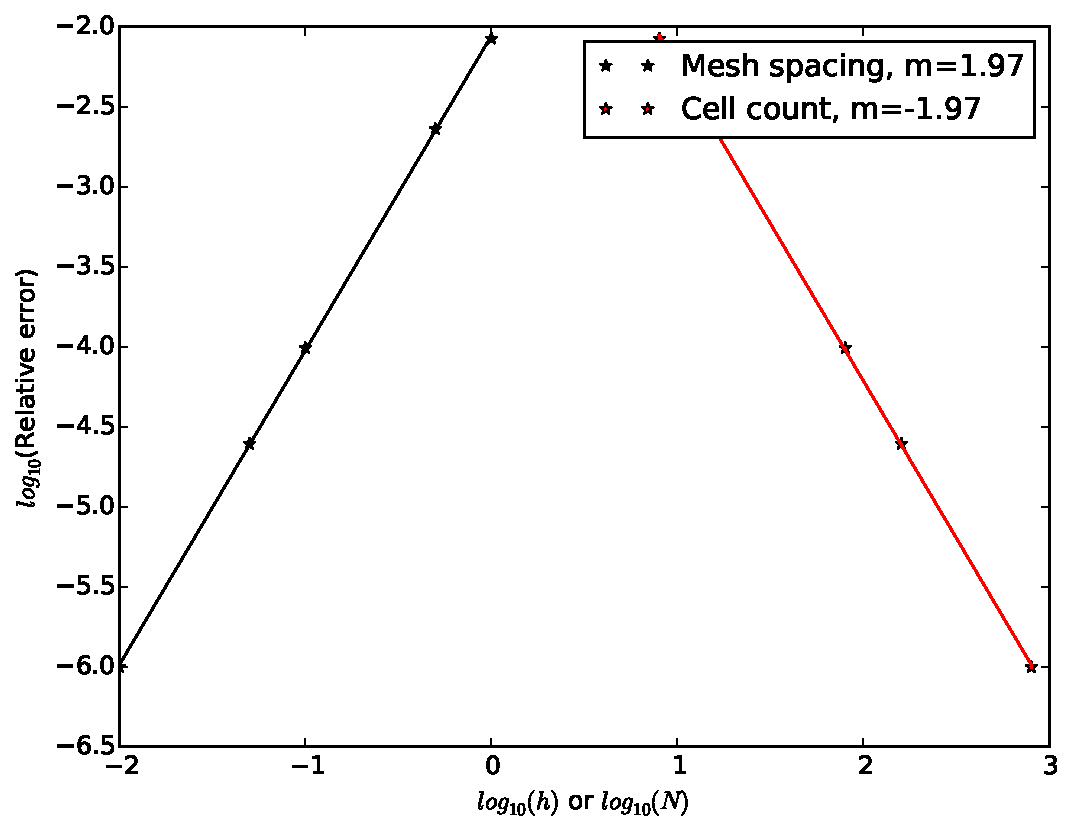
\includegraphics[width=10cm]{Question4.pdf}
  \caption{Relative error as a function of mesh spacing \(h\) and number of elements \(N\). The slopes \(m\) of each line are given in the legend.}
\end{figure}

\circled{5}\newline

\begin{enumerate}
\item We assume that neutron-neutron interactions are negligible. This assumption is perhaps the most important to the actual solution and numerical implementation of the transport equation, since otherwise the transport equation would be nonlinear, which brings significantly more difficulty in terms of analytical and numerical solution. Neutron-neutron interactions are \textit{very} scarce, and hence this approximation is also a very good approximation.
\item We assume that neutrons travel in straight lines between collisions. Because neutrons are neutral, the only body force acting on them that could cause them to move in non-straight lines is gravity. Because the mass of a neutron is very small, however, gravitational effects on the path of a neutron are negligible, and hence can be neglected. This approximation greatly simplifies the streaming term.
\item We neglect quantum and relativistic effects. Spin, parity, etc. are all neglected. Experience has shown this to be a good approximation, and greatly simplifies the transport equation by avoiding the need to include additional independent variables such as parity.
\item We assume neutrons are point particles. Then, the transport equation is an equation in seven variables \(x, y, z, t, E, \theta, \phi\), and we don't need to include an additional variable to represent how a neutron has rotated about its center of mass. Because neutrons are so small, this assumption does not introduce significant error.
\item We assume that material properties are isotropic, such that cross sections are not functions of \(\hat{\Omega}\). Most materials are isotropic due to the random orientation of grains, and hence this is a fairly good approximation.
\item For most general-purpose calculations, the cross sections are taken as independent of time because they change on such long length scales that a numerical simulation would be more effective in solving static, pseudo steady-state problems. This allows burnup calculations to be performed as a series of steps without continuous simulation, which reduces the computational cost significantly.
\end{enumerate}

\circled{8}\newline

The lowest energy isolated resonance is important in selecting the group structure to be used for multi-group calculations, since it would be best to create an energy group that contains the entire resonance, rather than splitting the resonance between multiple energy groups. For the purpose of determining the lowest isolated resonance, the \((n,\textrm{total})\) cross section is used, and a resonance is interpreted as any ``bump'' or peak in the cross section plot above the \(1/v\) dependence at low energies. For example, the cross section plot for U-235 is shown in Fig. \ref{fig:U235}. As can be seen, the lowest energy resonance occurs at approximately 2.7E-1 eV. Though not shown, similar plots were obtained for the other nuclides to fill out Table \ref{table:2}.

\begin{figure}[H]
  \centering
  \includegraphics[width=10cm]{U235.pdf}
  \caption{(n,total) cross section for U-235.}
  \label{fig:U235}
\end{figure}

\begin{table}[H]
\caption{Lowest isolated resonances of nuclides of interest from http://www.nndc.bnl.gov/sigma/.}
\centering
\begin{tabular}{l c}
\hline\hline
Nuclide & Lowest isolated resonance (eV)\\ [0.5ex]
\hline
U-235 & \(0.27\)\\
U-238 & \(6.40\)\\
Pu-239 & \(0.27\)\\
Pu-240 & \(1.00\)\\
Pu-241 & \(0.24\)\\
Pu-242 & \(2.60\)\\
\hline
\end{tabular}
\label{table:2}
\end{table}

\end{document}